\subsection{Filterspezifikation}

Beim zu realisierenden Stubfilter handelt es sich um ein Tiefpass-Filter 5. Ordnung, mit einer Grenzfrequenz (Passband) $f_C = 0.8GHz $ und einer Bezugsfrequenz $f_{\frac{\lambda}{4}} = 2GHz$. Die Bezugsfrequenz $f_{\frac{\lambda}{4}}$ definiert die Länge l der gleich langen Leitungsstücke uns ist folglich:

\begin{equation*}
l = \frac{\lambda}{4} = \frac{c}{4 \cdot f} = \frac{300\cdot 10^6 \lbrack\frac{m}{s}\rbrack}{4 \cdot 2 \lbrack GHz \rbrack} =37.5 \lbrack mm \rbrack
\end{equation*}

Das Stubfilter wird von einem Prototypfilter (Tiefpass 5. Ordnung) 
mit den Elementwerte $g_0$ bis $g_6$ abgeleitet.

\begin{figure}[h!]
\centering
 	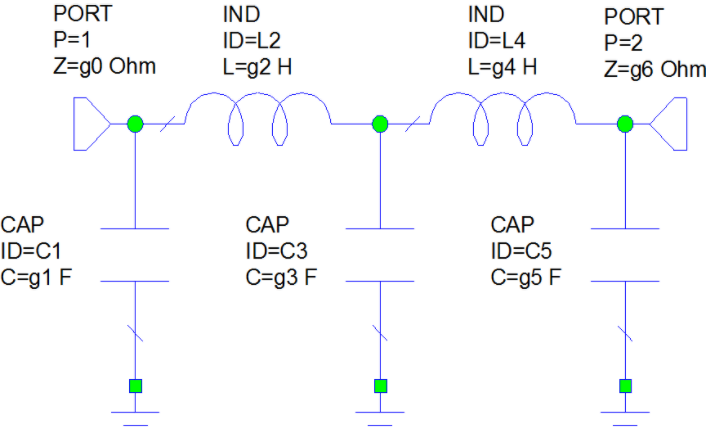
\includegraphics[width=0.5\textwidth]{Topologie_Prototyp.png}
 	\caption{Topologie des Prototypfilters}
 	\label{fig:Topologie_Prototyp.png}
\end{figure}

\begin{mdframed}
\begin{equation*} 
\begin{array}{rclcl} 
g_0 & = & 1 \\ 
g_1 & = & 0.973 \\ 
g_2 & = & 1.372 \\ 
g_3 & = & 1.803 \\ 
g_4 & = & 1.372 \\ 
g_5 & = & 0.973 \\ 
g_6 & = & 1 \\ 
\end{array} 
\end{equation*} 
\end{mdframed}

Durch eine Simulation in Mirowave Office (MWO) kann gezeigt werden, dass es sich beim Prototypfilter um ein Chebyshev Filter des Typs 1 handelt, weil das Filter im Passband einen Equirippel und im Stopband keinen Rippel aufweist. Dies wird aus der Übersichtdarstellung in Abb. \ref{fig:Ovw_Prototyp} ersichtlich, wo gleichzeitig die Einfügedämpfung S21 und die Reflexion S11 des simulierten Prototypfilters zu sehen ist.

\begin{figure}[h!]
\centering
 	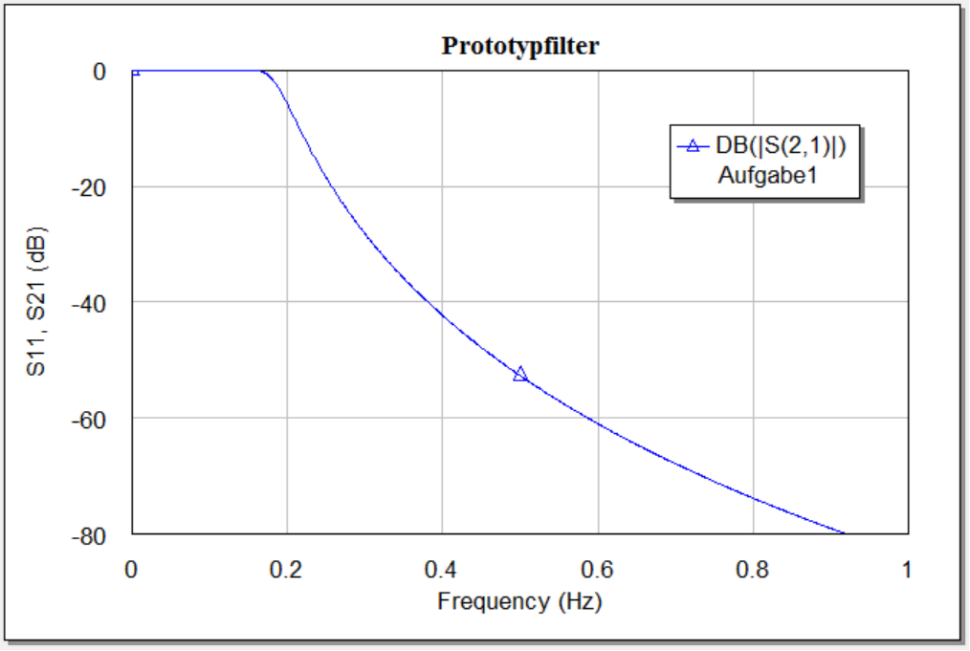
\includegraphics[width=0.5\textwidth]{Ovw_Prototyp.png}
 	\caption{Übersichtsdarstellung des Prototypfilters}
 	\label{fig:Ovw_Prototyp}
\end{figure}

Durch einen Zoom der Einfügedämpfung S21 in Abb. \ref{fig:Prototyp_Passbandrippel} wird der Equirippel des Passbands, sowie die erwartete Grenzfrequenz von $\omega_C = 1$  ersichtlich.

\begin{mdframed}
\begin{equation*} 
\begin{array}{rclcl} 
Equirippel & = & -0.04355 dB \\ 
\omega_C & = & 1 \\ 
f_C & = & 0.1592 Hz \\ 
\end{array} 
\end{equation*} 
\end{mdframed}

\begin{figure}[h!]
\centering
 	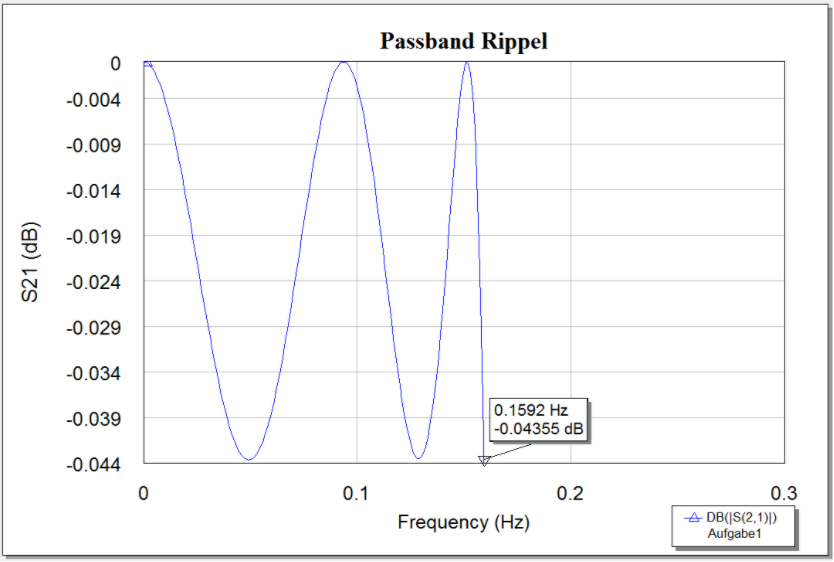
\includegraphics[width=0.5\textwidth]{Prototyp_Passbandrippel.png}
 	\caption{Equirippel im Passband}
 	\label{fig:Prototyp_Passbandrippel}
\end{figure}

Der vollständigkeit halber, wird auch noch die Reflexion S11 in Abb. 


Beim zu realisierende Stubfilter soll von einem Prototyp-Filter mit den folgenden Elementwerten ausgegange werden.
